\documentclass[10pt]{article}         % the type of document and font size (default 10pt)
\usepackage[margin=1.0in]{geometry}   % sets all margins to 1in, can be changed
\usepackage{moreverb}                 % for verbatimtabinput -- LaTeX environment
\usepackage{url}                      % for \url{} command
\usepackage{amssymb}                  % for many mathematical symbols
\usepackage[pdftex]{lscape}           % for landscaped tables
\usepackage{longtable}                % for tables that break over multiple pages
\usepackage[utf8]{inputenc}           % UTF8 characters
\usepackage[T1]{fontenc}
\usepackage{textcomp}
\usepackage[english]{babel}
\usepackage{float}                    % Position of figure, table
\usepackage{enumitem}                 % Alphabet list
\usepackage{makecell}                 % Customize cells in a table
\usepackage{amsmath}
\usepackage{amsfonts}
\usepackage{amssymb}
\usepackage{mathtools}
\usepackage{graphicx}
\usepackage{babel,blindtext}
\graphicspath{ {../output/} }
\DeclarePairedDelimiter{\ceil}{\lceil}{\rceil}
\renewcommand{\baselinestretch}{1.5}
\title{COCS 6323: Statistical Methods in Research \\ Group Project} % to specify title
\author{Group <number> \\
        Department of Computer Science\\
        University of Houston}         % to specify author(s)
\usepackage{Sweave}
\begin{document}                      % document begins here
\Sconcordance{concordance:ProjectReport.tex:ProjectReport.Rnw:%
1 31 1 1 0 13 1}
\Sconcordance{concordance:ProjectReport.tex:././sections/contribution2.Rnw:ofs 46:%
1 11 1}
\Sconcordance{concordance:ProjectReport.tex:ProjectReport.Rnw:ofs 58:%
47 2 1}
\Sconcordance{concordance:ProjectReport.tex:././sections/section4.Rnw:ofs 61:%
1 9 1}
\Sconcordance{concordance:ProjectReport.tex:ProjectReport.Rnw:ofs 71:%
51 2 1}
\Sconcordance{concordance:ProjectReport.tex:././sections/sectionT2.Rnw:ofs 74:%
1 32 1}
\Sconcordance{concordance:ProjectReport.tex:ProjectReport.Rnw:ofs 107:%
55 2 1}
\Sconcordance{concordance:ProjectReport.tex:././sections/sectionT3.Rnw:ofs 110:%
1 65 1}
\Sconcordance{concordance:ProjectReport.tex:ProjectReport.Rnw:ofs 176:%
59 4 1}


\setkeys{Gin}{width=1.0\textwidth}

\maketitle              % makes the title

\newpage
\tableofcontents        % inserts TOC (section, sub-section, etc numbers and titles)
\listoftables           % inserts LOT (numbers and captions)
\listoffigures          % inserts LOF (numbers and captions)

\newpage
\section{Contribution}
% !Rnw root = ../ProjectReport.Rnw
\begin{table}[h]
\begin{tabular}{|l|l|}
\hline
\textbf{Member} & \textbf{Contribution} \\ \hline
Brad & 3A 3B 3C S2\\ \hline
Tung Huynh & 2A 2B S3 S4\\ \hline
Yifan & 3D 3E 3F S1\\ \hline
\end{tabular}
\caption{Contribution of group member}
\label{tbl:contribution}
\end{table}

\newpage
\section{Figure 2A}
% !Rnw root = ../ProjectReport.Rnw
\begin{figure}[!htb]
  \minipage{0.32\textwidth}
    \textbf{1990}\\
    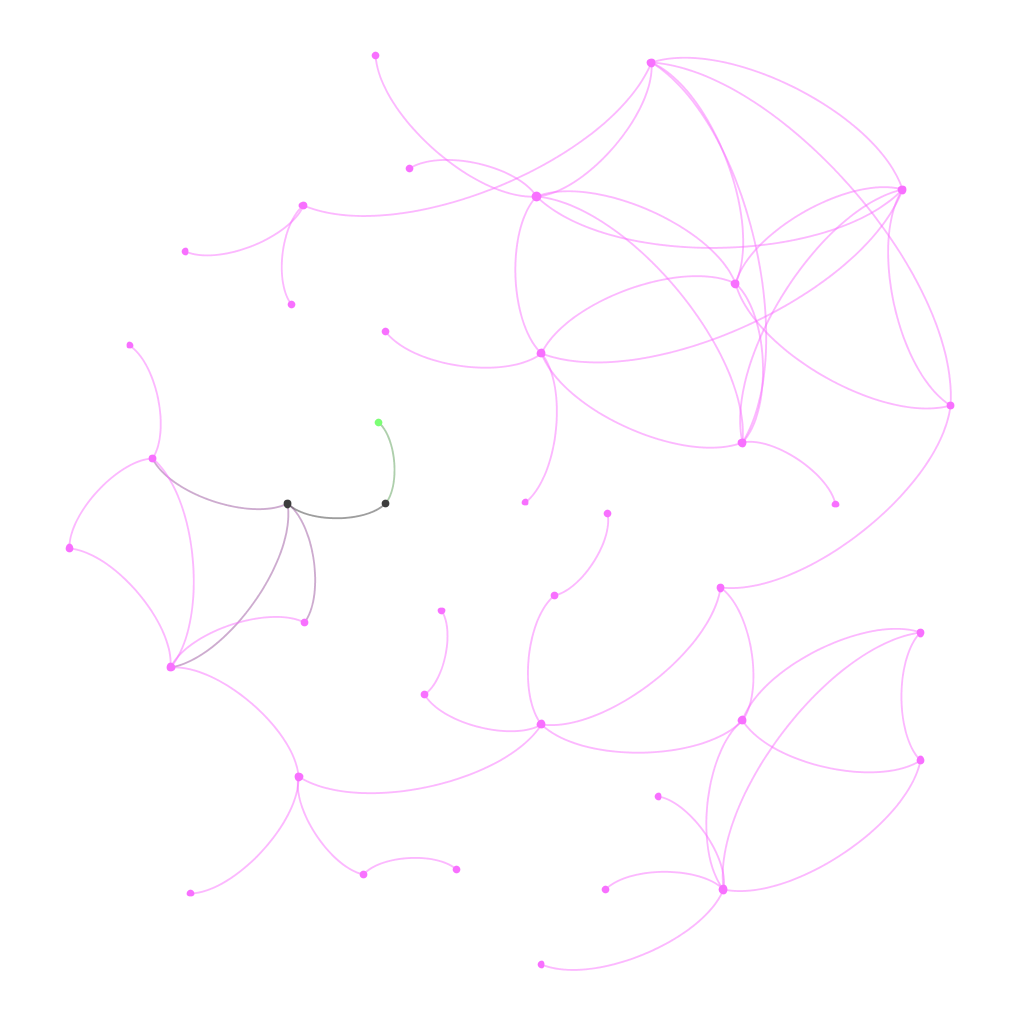
\includegraphics[width=5cm, height=5cm]{Fig2A1990.png}
  \endminipage\hfill
  \minipage{0.32\textwidth}
    \textbf{1995}\\
    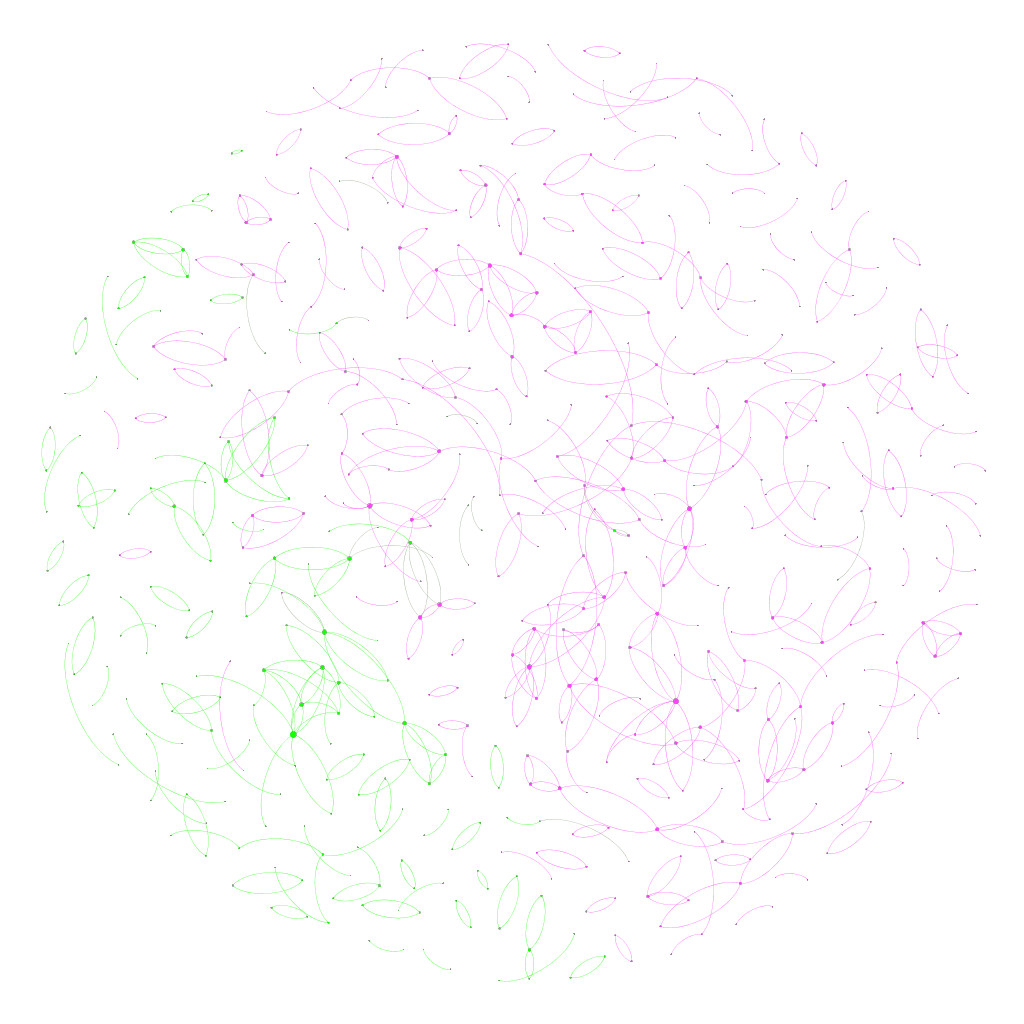
\includegraphics[width=5cm, height=5cm]{Fig2A1995.png}
  \endminipage\hfill
  \minipage{0.32\textwidth}%
    \textbf{2000}\\
    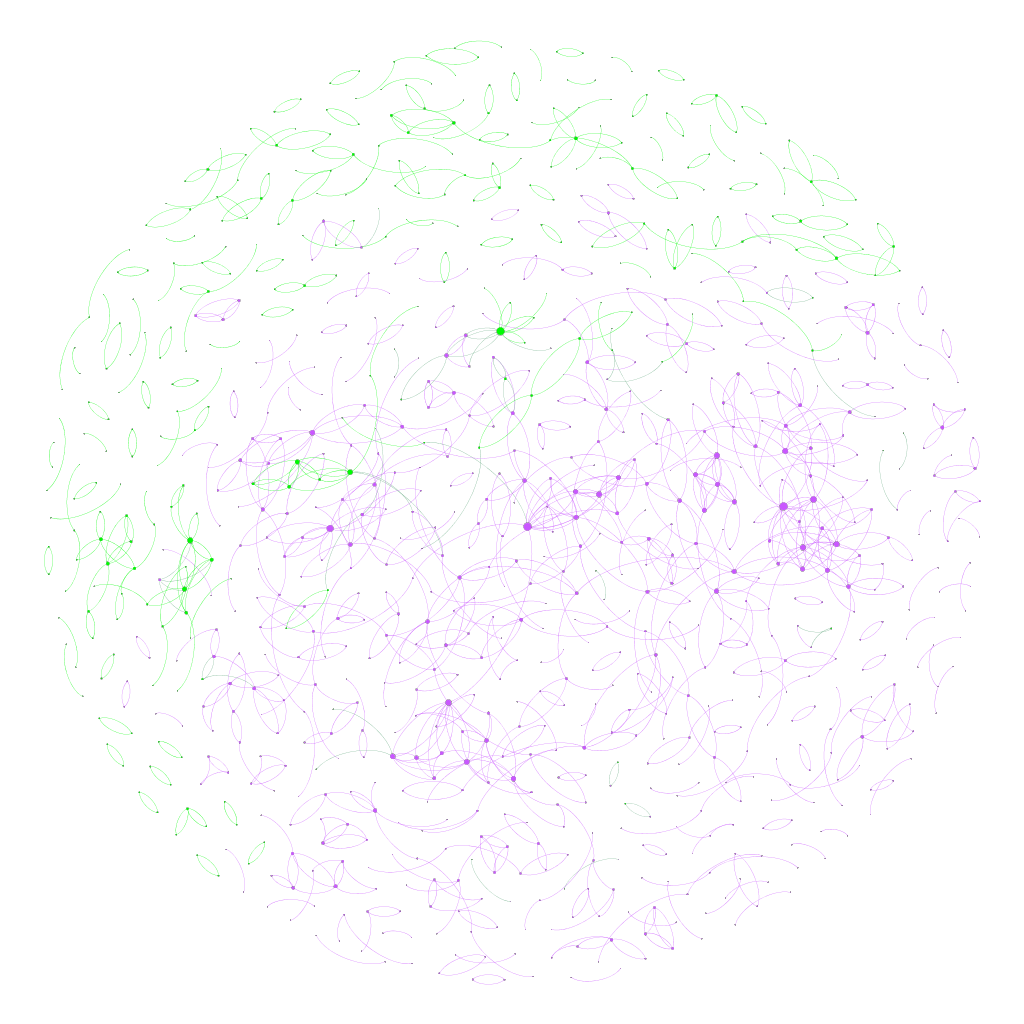
\includegraphics[width=5cm, height=5cm]{Fig2A2000.png}
  \endminipage\hfill
  \minipage{0.32\textwidth}
    \textbf{2005}\\
    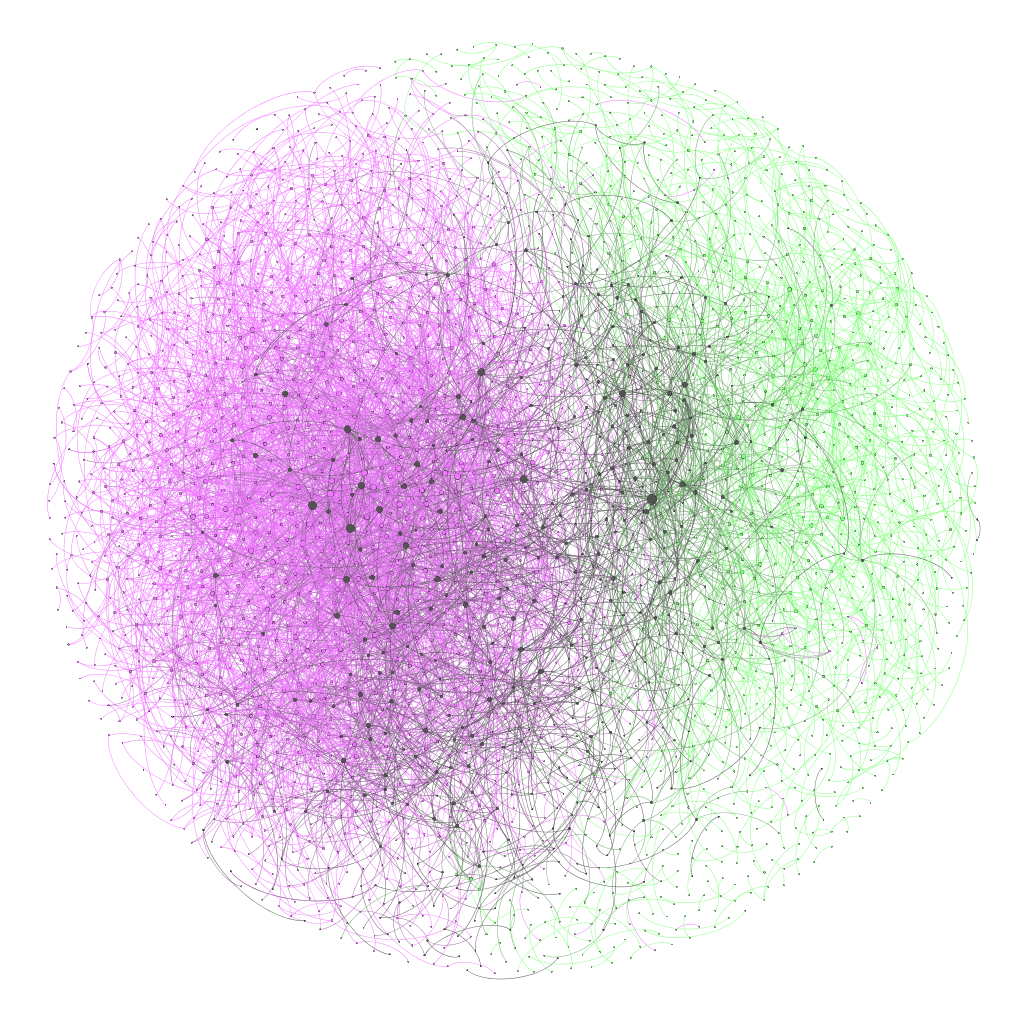
\includegraphics[width=5cm, height=5cm]{Fig2A2005.png}
  \endminipage\hfill
  \minipage{0.32\textwidth}
    \textbf{2010}\\
    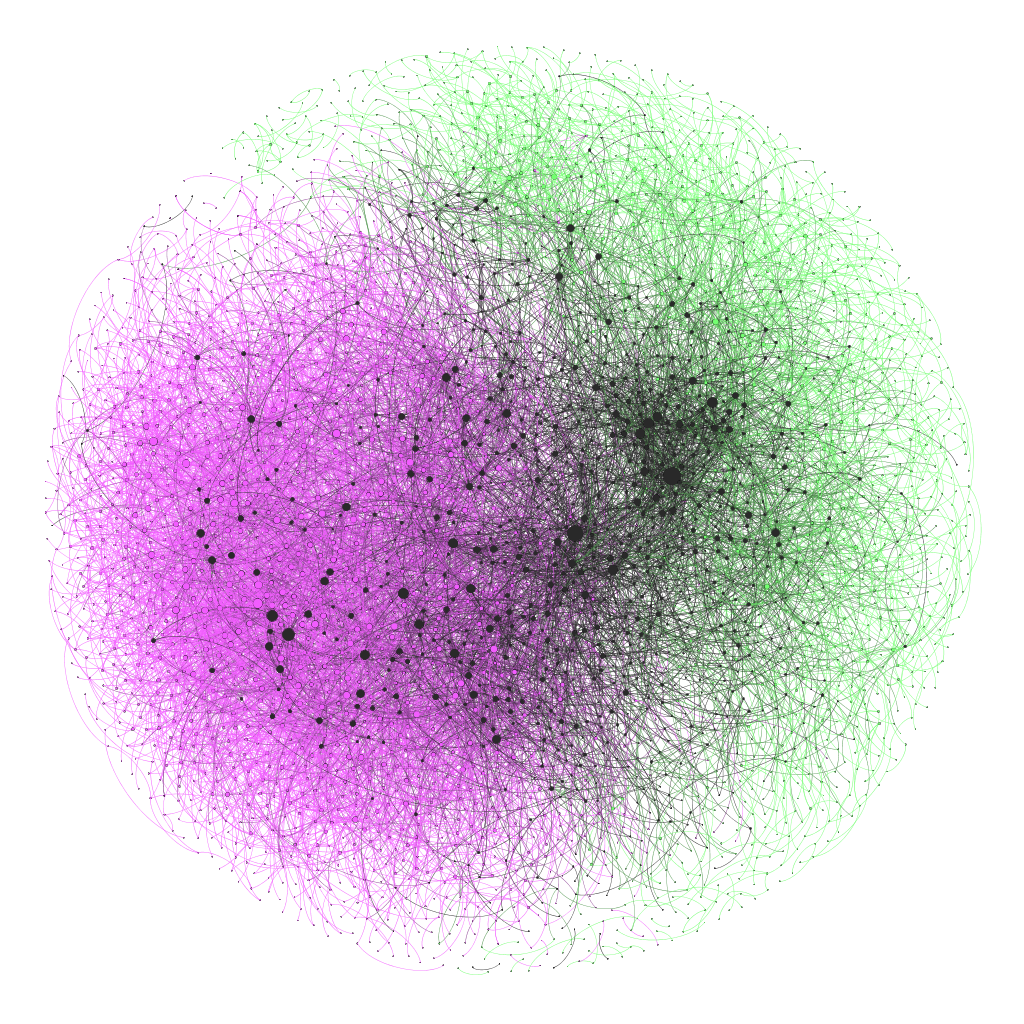
\includegraphics[width=5cm, height=5cm]{Fig2A2010.png}
  \endminipage\hfill
  \minipage{0.32\textwidth}%
    \textbf{2015}\\
    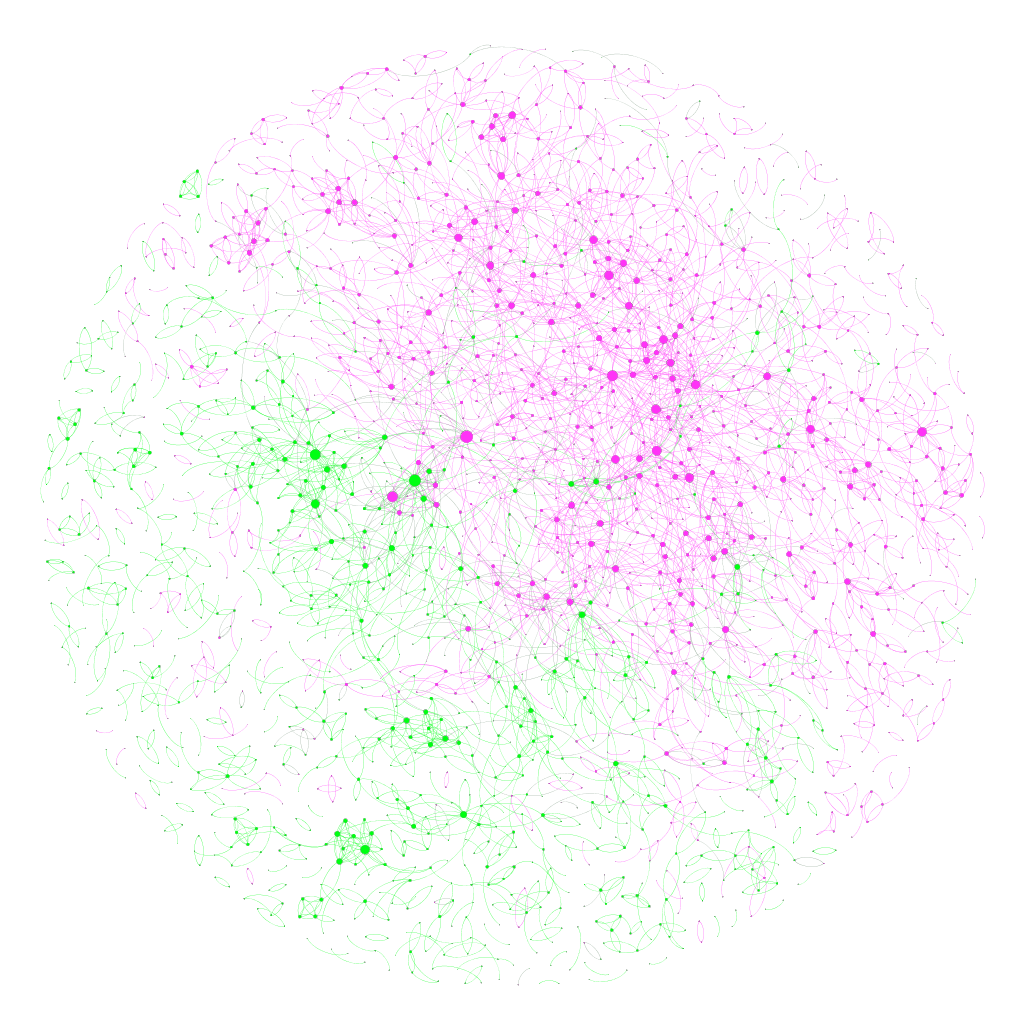
\includegraphics[width=5cm, height=5cm]{Fig2A2015.png}
  \endminipage
  \caption{Growth of cross-disciplinary social capital}
  \label{fig:2A}
\end{figure}

This figure depicts the evolution of the giant component in the U.S. biology-computing network of collaborations. It consists of six consecutive periods from 1990 to 2015. Each period illustrates the collaborations of the two departments in five previous years. While green and magenta nodes represent faculty $F_i$ in $BIO$ and $CS$ department, respectively; black vertices represent faculty $F_i$ that published at least one cross-disciplinary publication. In this figure, node size is proportional to the logarithm of the degree centrality, the total number of collaborations of the faculty.

In the first network of the year 1990, the giant component only consists of links between CS nodes. In the period from 1900 to 2005, in which the HGP happens, the networks represent the establishment of cross-disciplinary collaborations. Finally, in the last period from 2005 to 2015, the giant component does not only expands in term of the number of collaborations and robustness, but it also notably illustrates the significant role of $XD$ group containing the largest nodes in the network.

\newpage
\section{Figure 2B}
% !Rnw root = ../ProjectReport.Rnw
\begin{figure}[!htb]
  \centering
  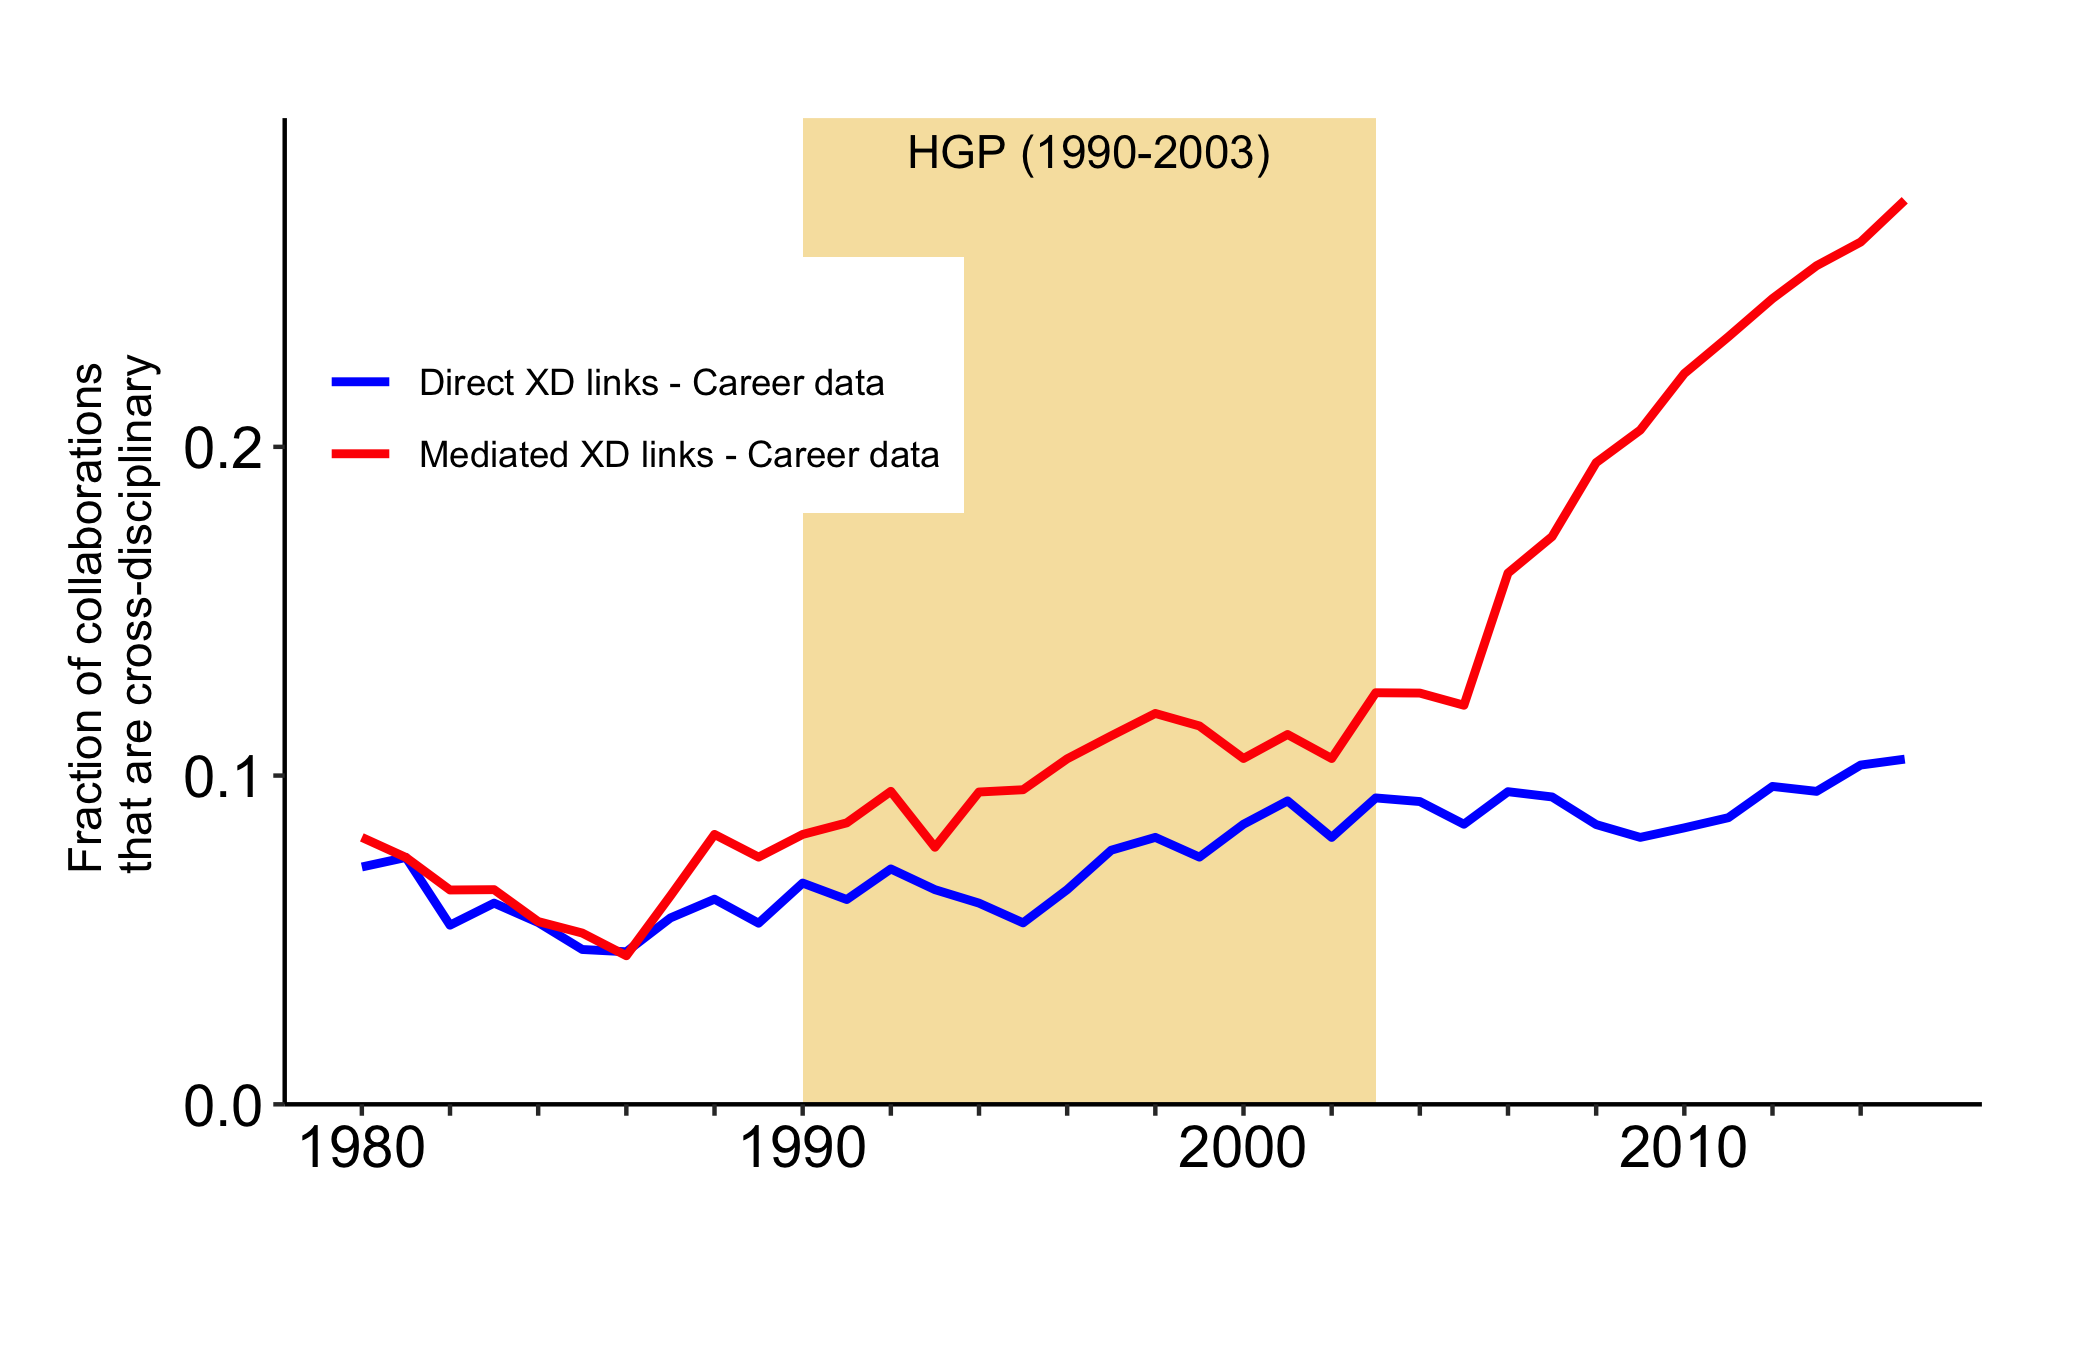
\includegraphics[width=10cm, height=7cm]{Fig2B.png}
  \caption{Evolution of the fraction of cross-disciplinary collaboration links}
  \label{fig:2B}
\end{figure}

This figure depicts the evolution of the fraction of collaboration links in the network that are cross-disciplinary. While blue line illustrate the direct $XD$ links, the red line represent the mediated $XD$ links by pollinators. The orange area in the middle annotates the HGP project period from 1990 to 2013.

\newpage
\section{Figure 3A}
% !Rnw root = ../ProjectReport.Rnw

\begin{figure}[!htb]
  \centering
  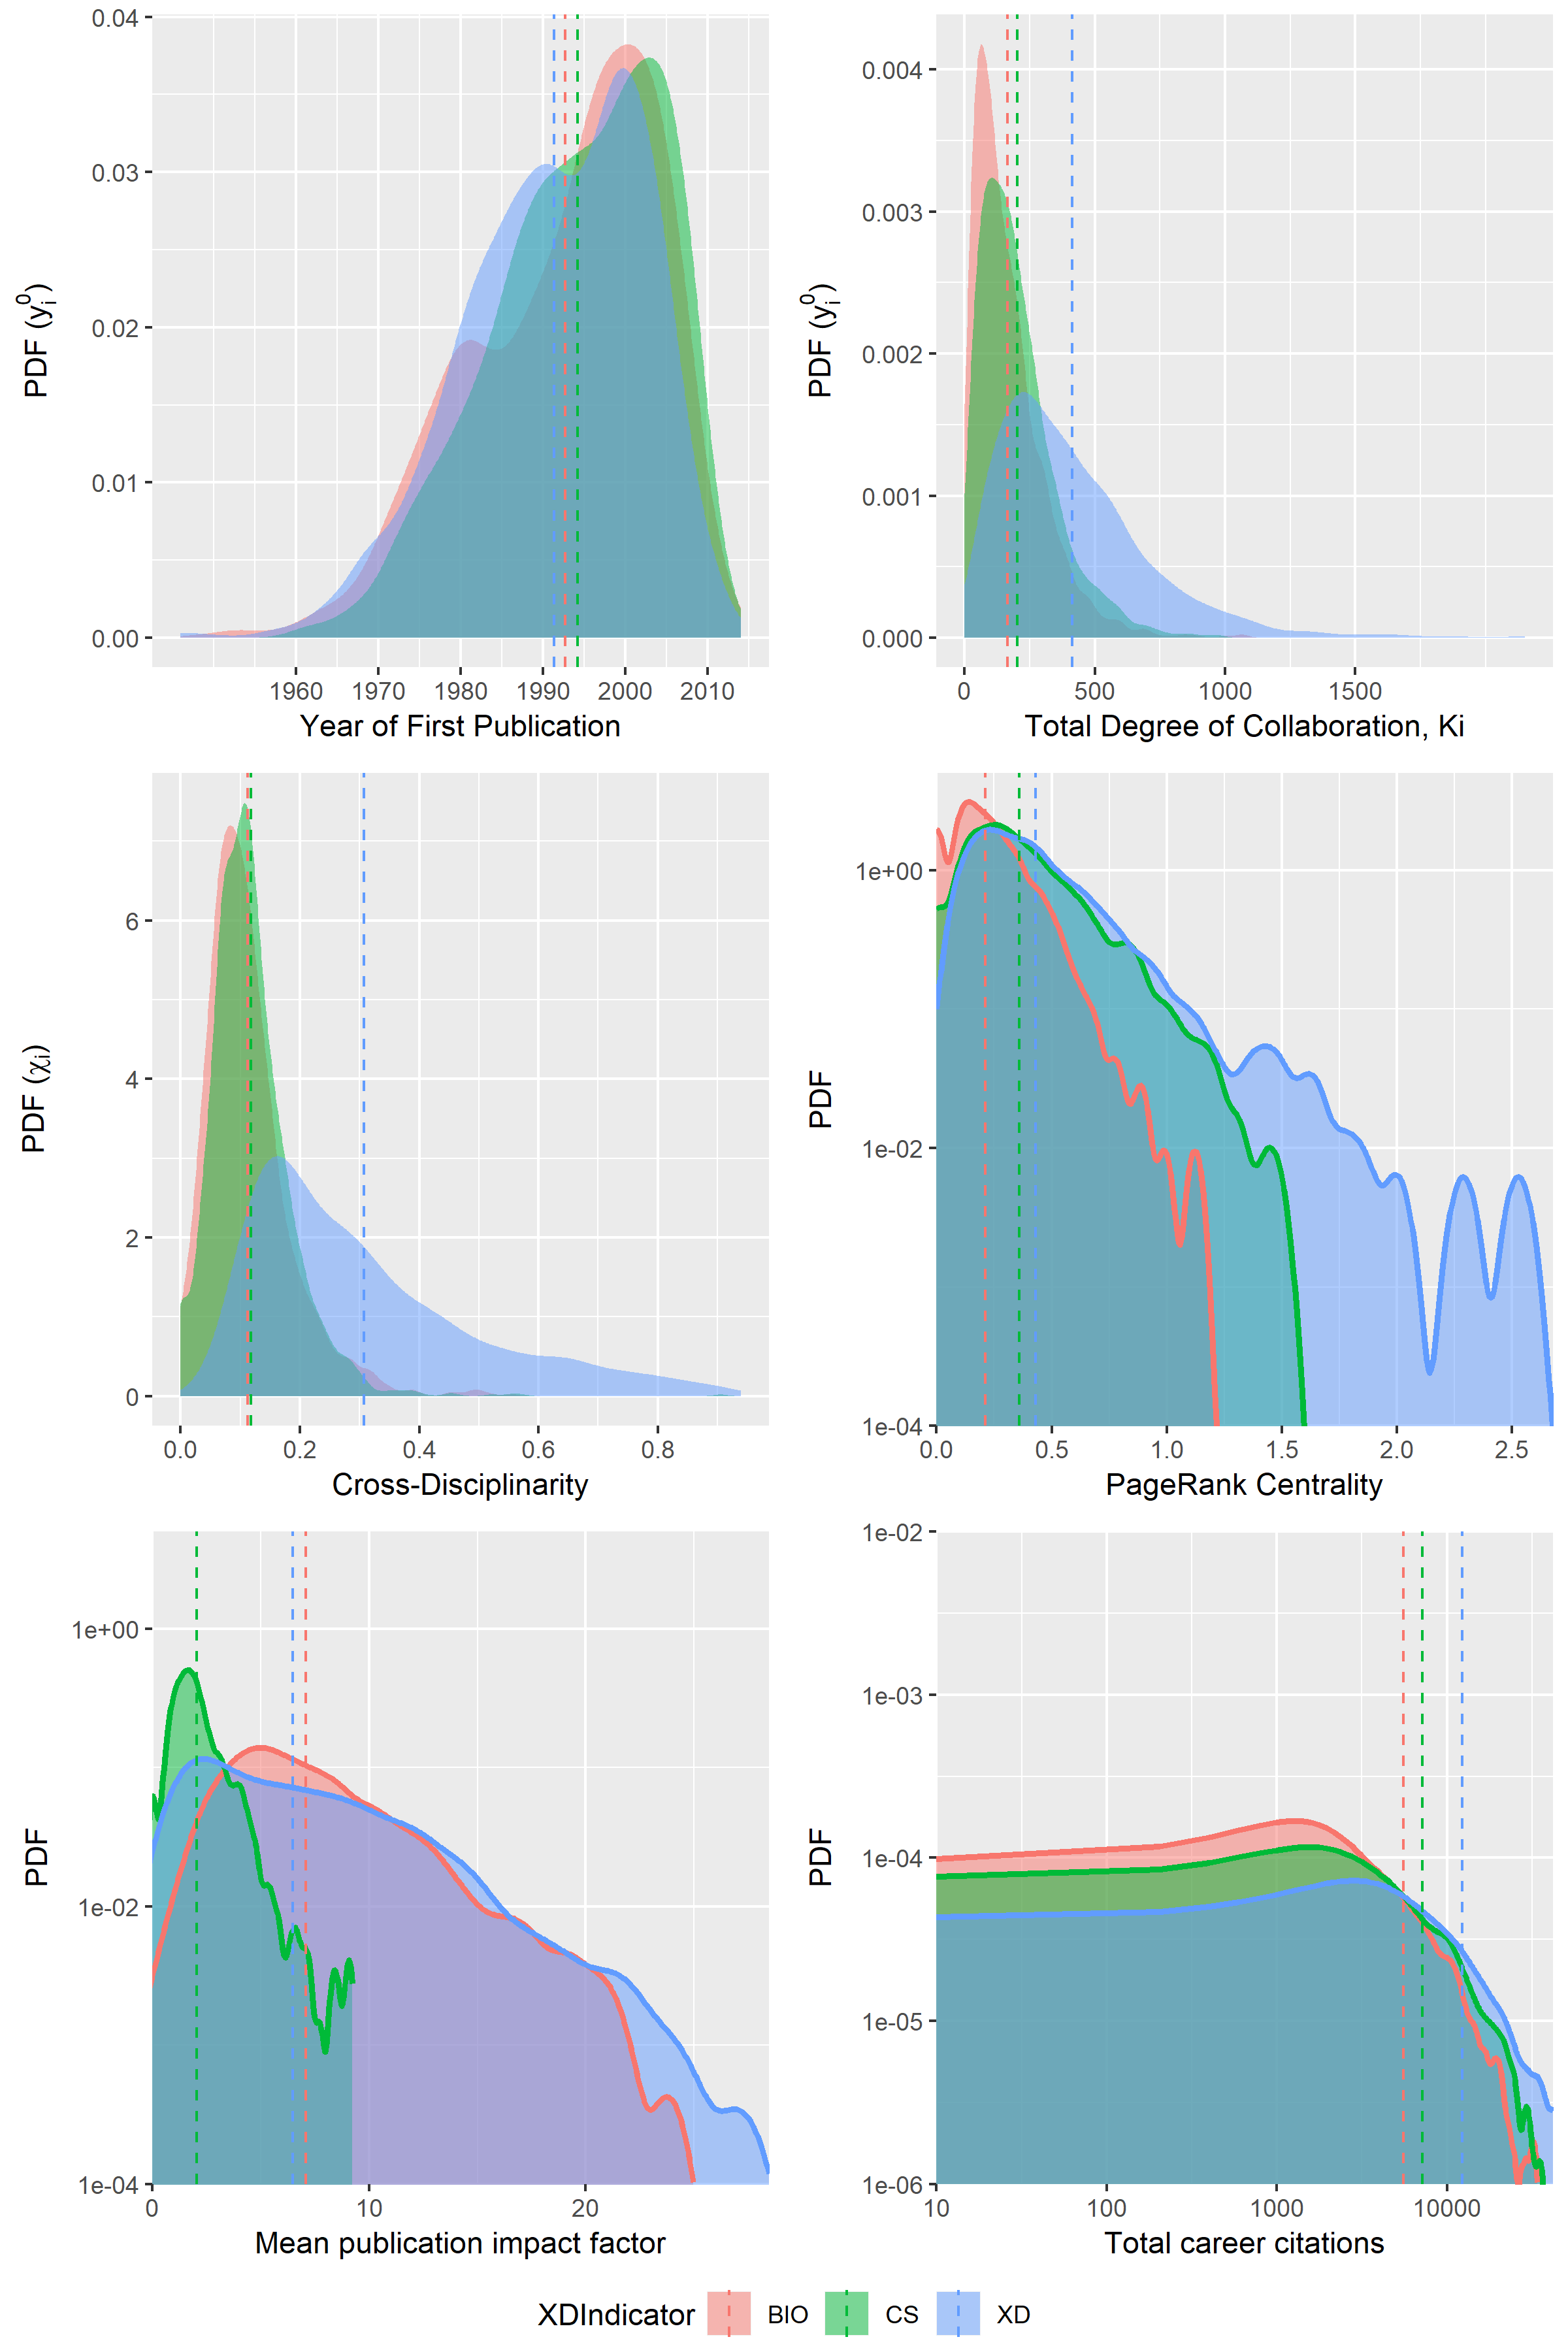
\includegraphics[width=10cm, height=7cm]{xd-project/plot3_all.png}
  \caption{Descriptive statistics of the career dataset}
  \label{Fig3}
\end{figure}

Figures 3 a-F, are probability distributions of the following data: year of first publication, total number of collaborators, the fraction of collaborators who are XD, PageRank centrality of professors within the network, and mean impact factor of the publication record of professors within the network. The data visualization above supports a conclusion that XD professors are more collaborative than BIO or CS specific professors. Figures 3B, C, and D show that XD professors are more collaborative than their single-discipline counterparts. XD professors are also shown to have greater total degrees of collaboration, a greater fraction of collaborators who themselves are XD, and higher overall PageRank centrality. XD professors also outperform BIO and CS in terms of mean publication impact factor. Figure 3A suggests that XD professors published their first paper in genomics on average before BIO and CS. 

\newpage
\section{Figure 3B}
% !Rnw root = ../ProjectReport.Rnw
Add the content of this section

\newpage
\section{Figure 3C}
% !Rnw root = ../ProjectReport.Rnw
Add the content of this section

\newpage
\section{Figure 3D}
% !Rnw root = ../ProjectReport.Rnw
Add the content of this section

\newpage
\section{Figure 3E}
% !Rnw root = ../ProjectReport.Rnw
Add the content of this section

\newpage
\section{Figure 3F}
% !Rnw root = ../ProjectReport.Rnw
Add the content of this section
Figures 3 a-F, are probability distributions of the following data: year of first publication, total number of collaborators, the fraction of collaborators who are cross-disciplinary, PageRank centrality of professors within the network, and mean impact factor of the publication record of professors within the network. The data visualization above supports a conclusion that cross-disciplinary professors (XDF) are more collaborative than biology or computer science specific professors. Figures 3B, C, and D show that cross-disciplinary professors are more collaborative than their single-discipline counterparts. Cross-disciplinary professors have greater total degrees of collaboration, a greater fraction of collaborators who themselves are cross-disciplinary, and higher overall PageRank centrality. Cross-disciplinary professors also outperform biologists and computer scientists in terms of mean publication impact factor. Figure 3A suggests that cross-disciplinary professors published their first paper in genomics on average before biologists and computer scientists. 

\newpage
\section{Supplementary S1}
% !Rnw root = ../ProjectReport.Rnw
Add your content here\\
Figure S1a depicts the ratio of the largest component other than the initial giant component within the F network. By randomly removing links, the robustness of the network is tested through the observation of the relative size of the remaining giant component to the next largest subnetwork. Error bars are fitted to points on the curve depicting mean and standard deviation. This ratio slowly declines until roughly ___, from this observation we can assert ____. Figure S1b shows when the network breaks up into significantly smaller subnetworks and the giant component itself degrades. This measured peak breaking point coincides with the steep decline observed in S1a, confirming that at this fraction of links removed, the ratio of giant component to next largest subnetwork declines as well. 

\newpage
\section{Supplementary S2}
% !Rnw root = ../ProjectReport.Rnw
\begin{figure}[!htb]
  \centering
  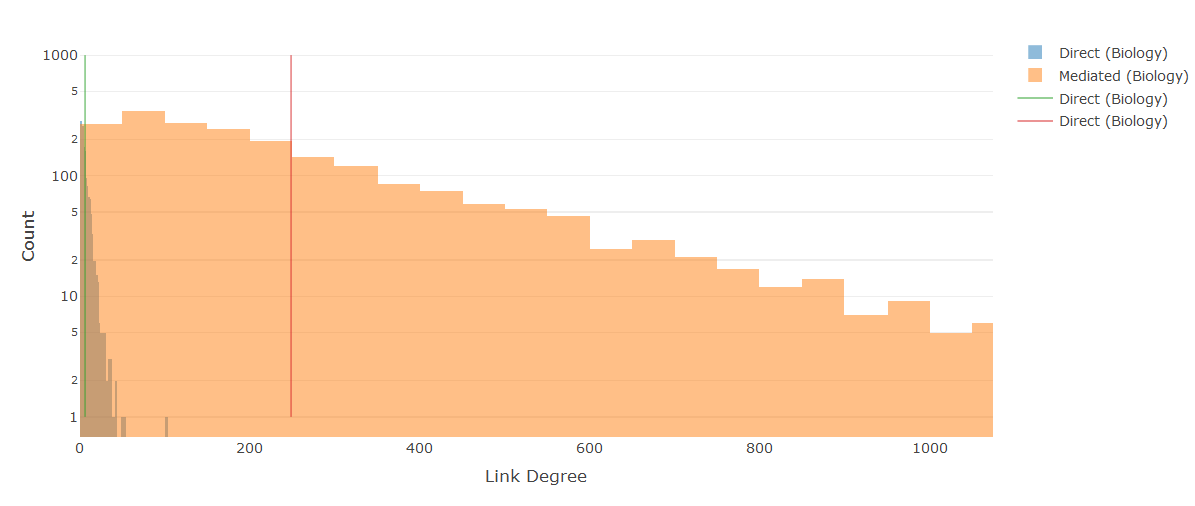
\includegraphics[width=11cm, height=5cm]{Fig2SA.PNG}
  \caption{Network Distributions for Direct and Mediated Associations of Biologists}
  \label{fig:S2A}
\end{figure}
\begin{figure}[!htb]
  \centering
  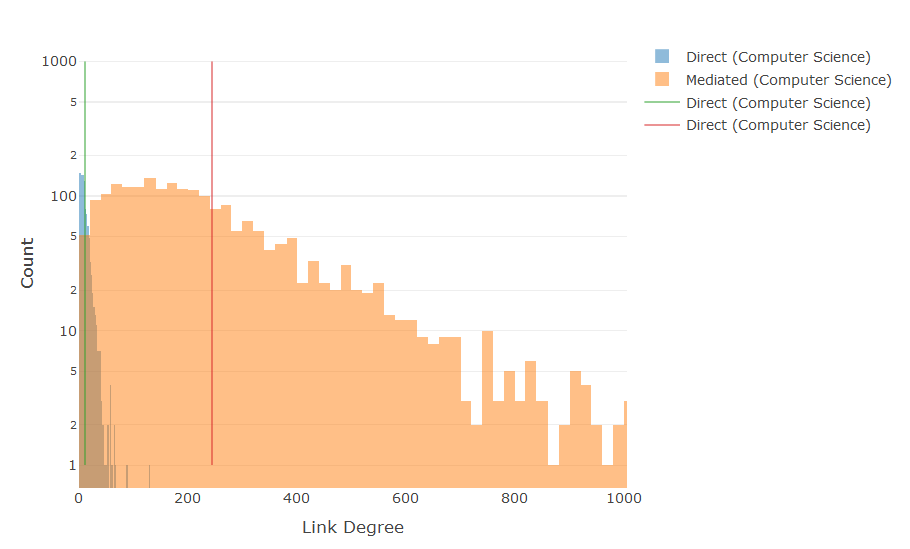
\includegraphics[width=10cm, height=7cm]{Fig2SB.PNG}
  \caption{Network Distributions for Direct and Mediated Associations of Computer Scientists}
  \label{fig:S2B}
\end{figure}
Figure S2 depicts the number of associations between professors within BIO departments (a), and CS departments (b) with other researchers studying genomics. The dark area shows counts of the direct connections between professors, while the lighter orange area shows counts of mediated connections. Vertical lines represent means of each distribution. Direct links are made when professors within the Fi dataset collaborate to publish a paper. Mediated links are established when professors have a collaborator who exists outside of Fi in common. The histograms above demonstrate the importance of the mediated connections, with regards to the robustness of the network. Thus, professors who are outside of the dataset at hand make an important impact on the social network studied here.  

\newpage
\section{Supplementary S3}
% !Rnw root = ../ProjectReport.Rnw
\begin{figure}[!htb]
  \minipage{0.32\textwidth}
    \textbf{Degree}\\
    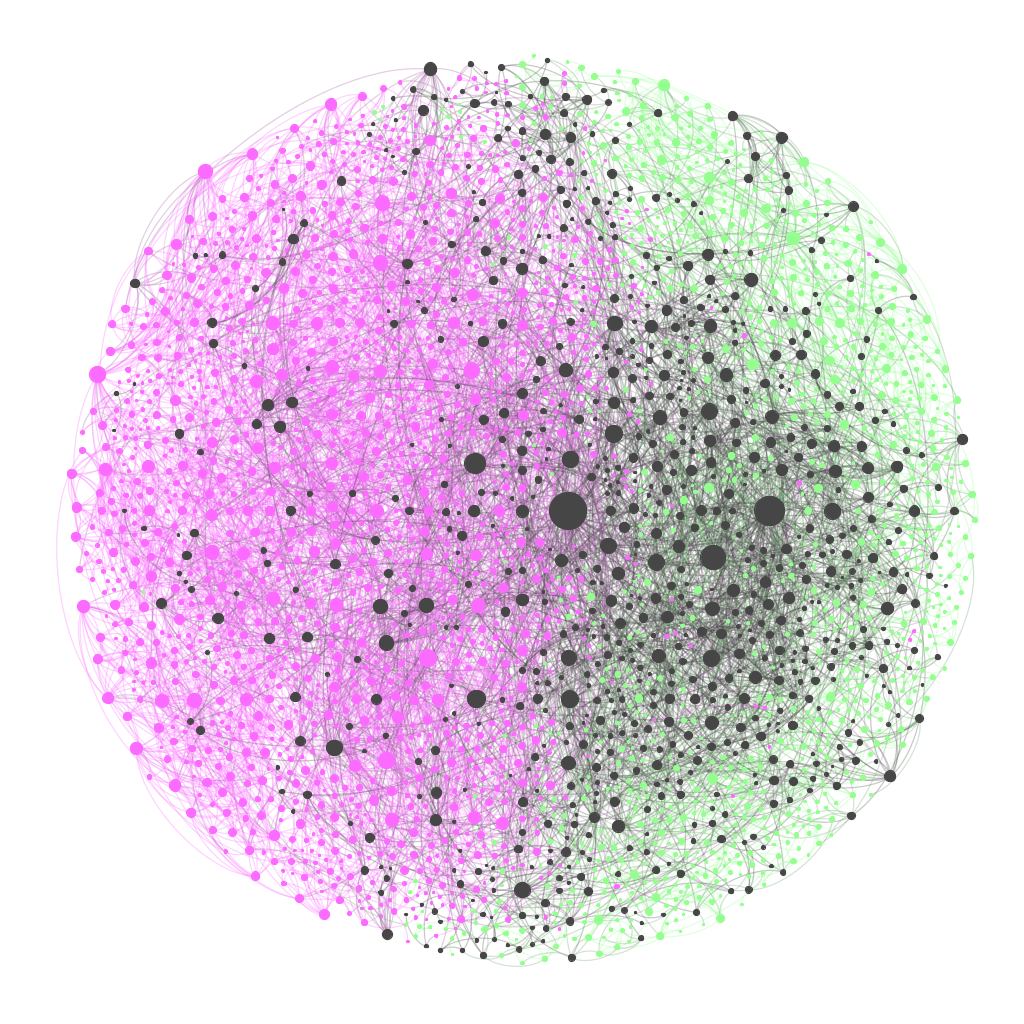
\includegraphics[width=5cm, height=5cm]{S3Degree.png}
  \endminipage\hfill
  \minipage{0.32\textwidth}
    \textbf{PageRank}\\
    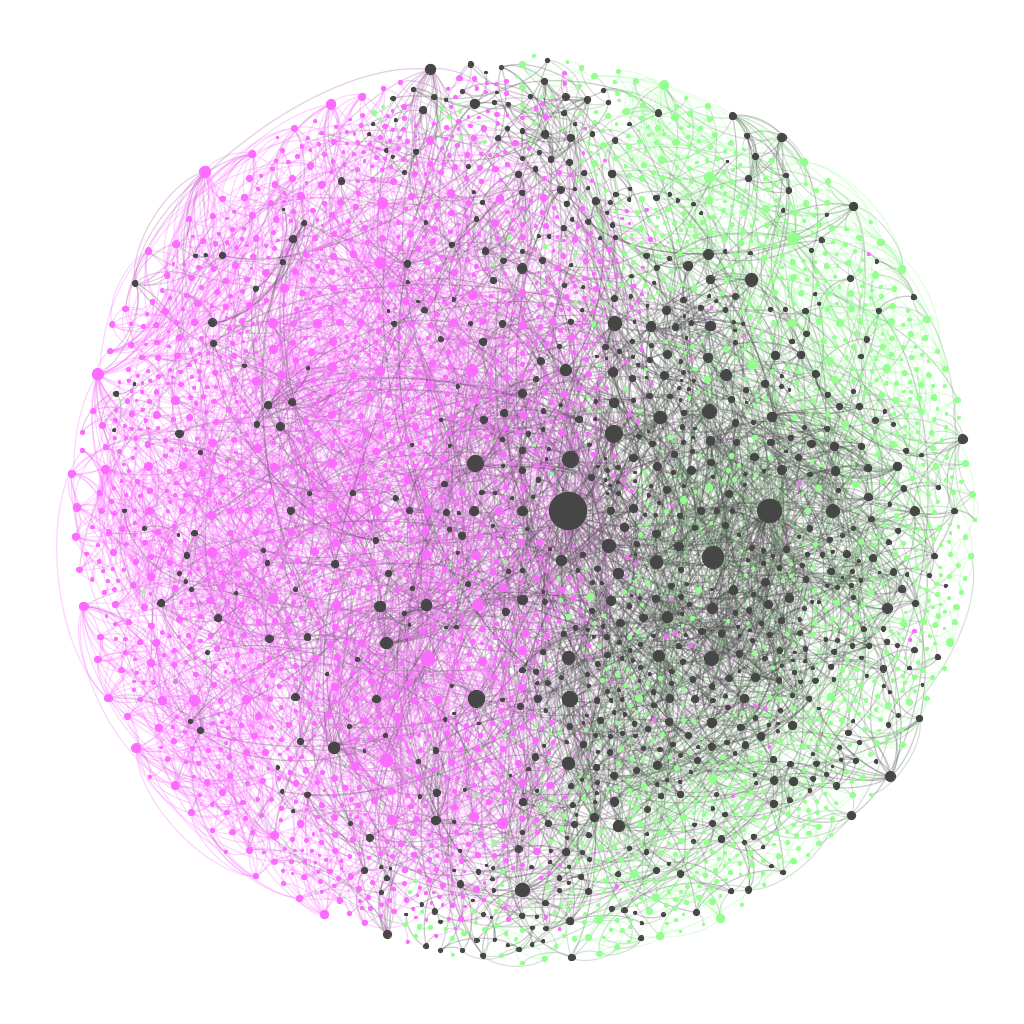
\includegraphics[width=5cm, height=5cm]{S3PageRank.png}
  \endminipage\hfill
  \minipage{0.32\textwidth}%
    \textbf{Betweenness}\\
    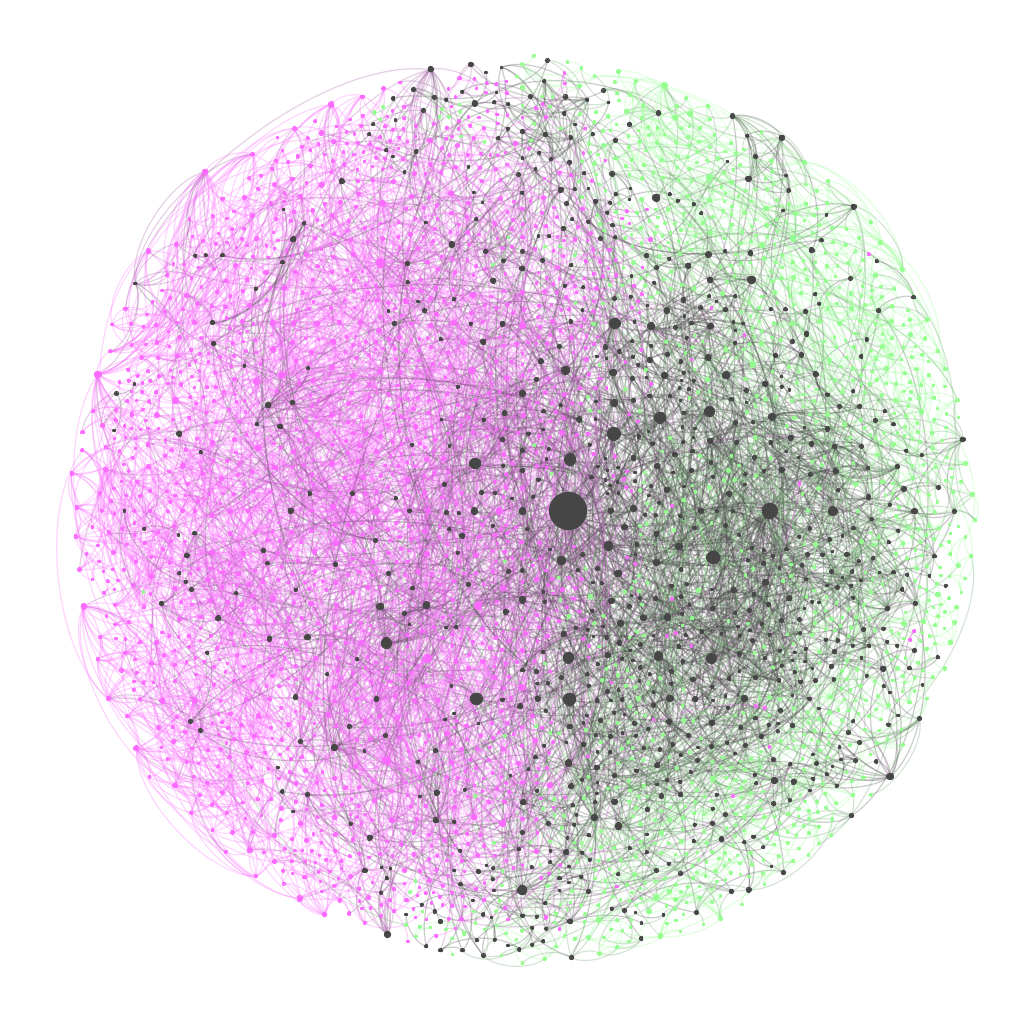
\includegraphics[width=5cm, height=5cm]{S3Betweeness.png}
  \endminipage
  \caption{Three perspectives on the centrality of $F_i$ in the direct collaboration network}
  \label{fig:s3}
\end{figure}

This figure shows the giant connected component of the faculty network using all data up to 2015 from three different perspectives. The position of nodes and links are unchanged in the three networks. And the node sizes change respectively to the three centrality measure including Degree, PageRank, and Betweenness.

While Degree centrality treats the importance of each node equally, PageRank takes into account the prominence of each faculty. Therefore, with the same number of links, a node size of faculty $F_i$ in the network using PageRank centrality measure changes to smaller or larger than its counterpart in the network using Degree centrality measure according to the prominence of his collaborators.

Besides, because the Betweenness centrality measures the number of shortest paths passing through a node, the network using this measure only emphasize on those nodes helping to increase the robustness of the whole network.

Remarkably, regardless of the change of centrality measure using in each network, the group of founders of HGP including Eric Lander always demonstrate their significant role of connecting the cross-disciplinary links with the highest central.

\newpage
\section{Supplementary S4}
% !Rnw root = ../ProjectReport.Rnw
\begin{figure}[!htb]
  \minipage{0.32\textwidth}
    \textbf{1990}\\
    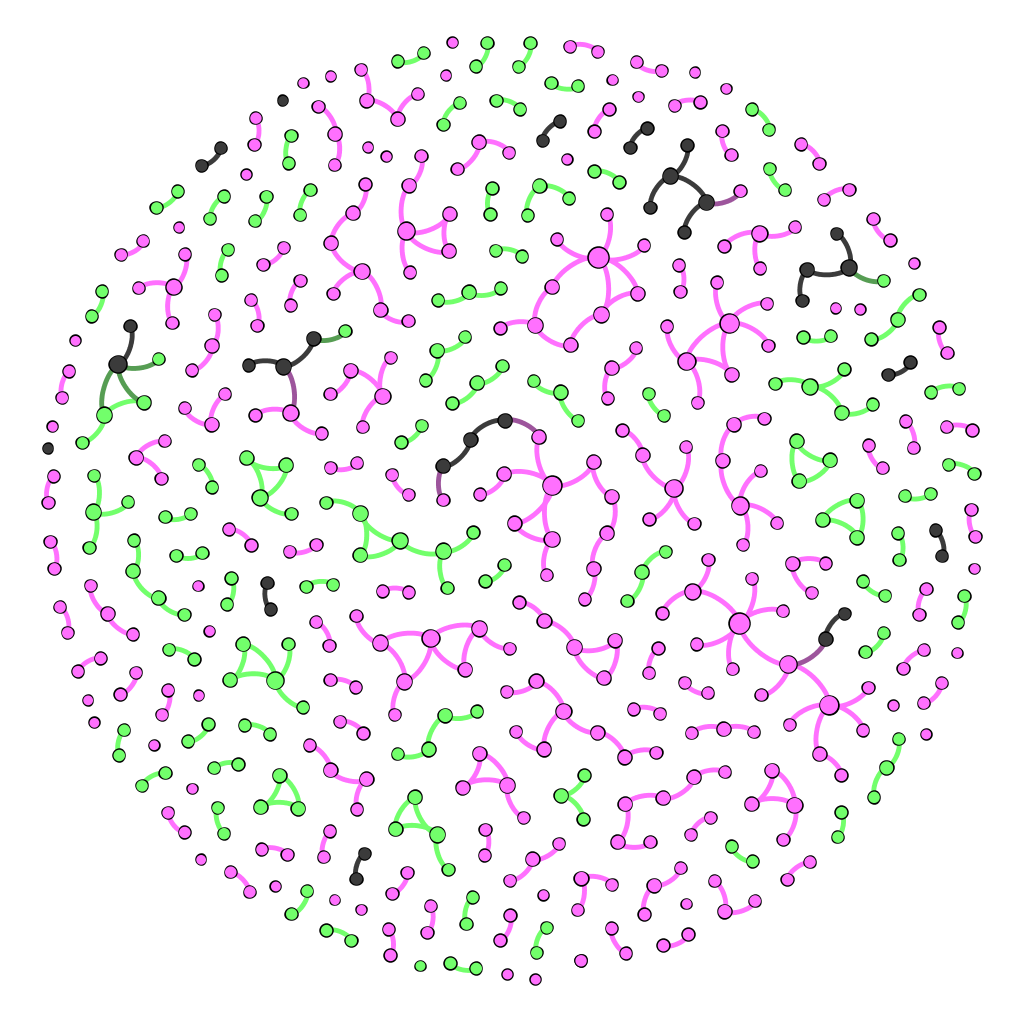
\includegraphics[width=5cm, height=5cm]{S41990.png}
  \endminipage\hfill
  \minipage{0.32\textwidth}
    \textbf{1995}\\
    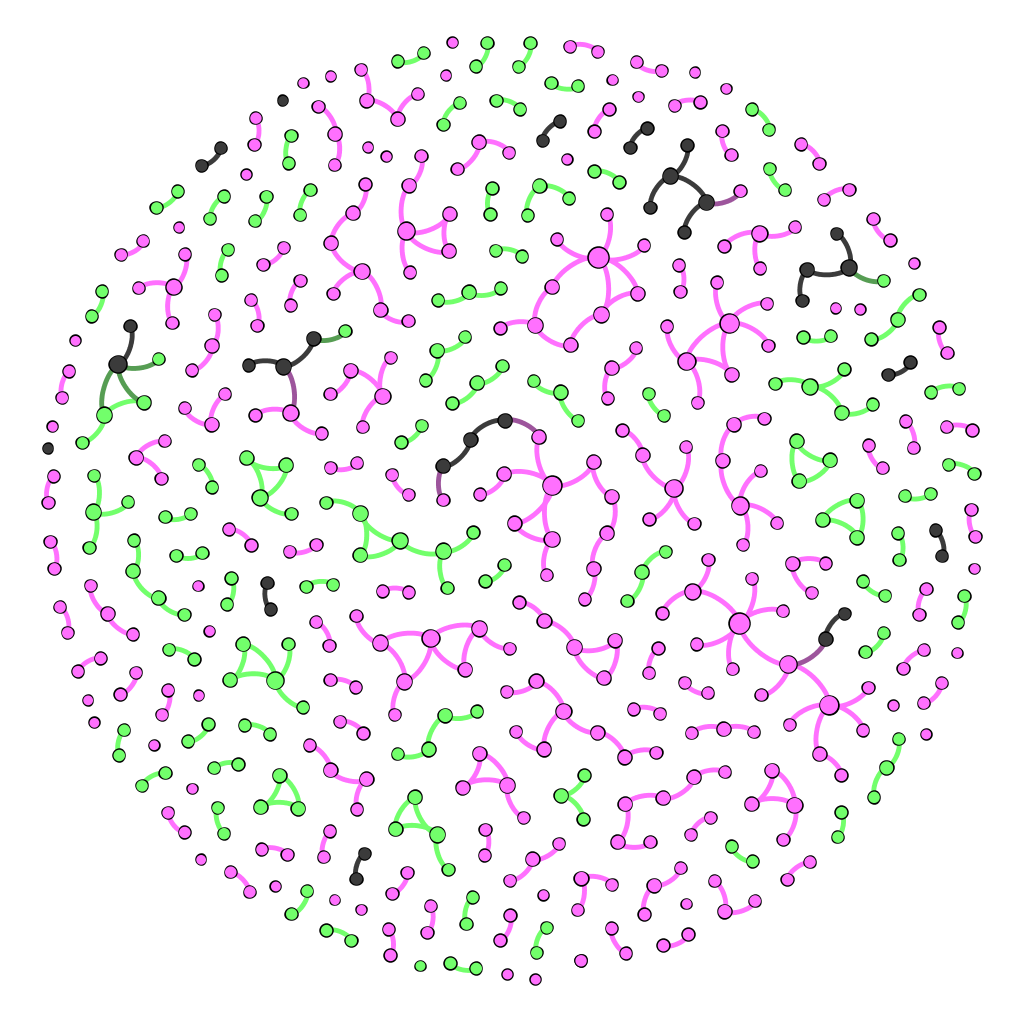
\includegraphics[width=5cm, height=5cm]{S41995.png}
  \endminipage\hfill
  \minipage{0.32\textwidth}%
    \textbf{2000}\\
    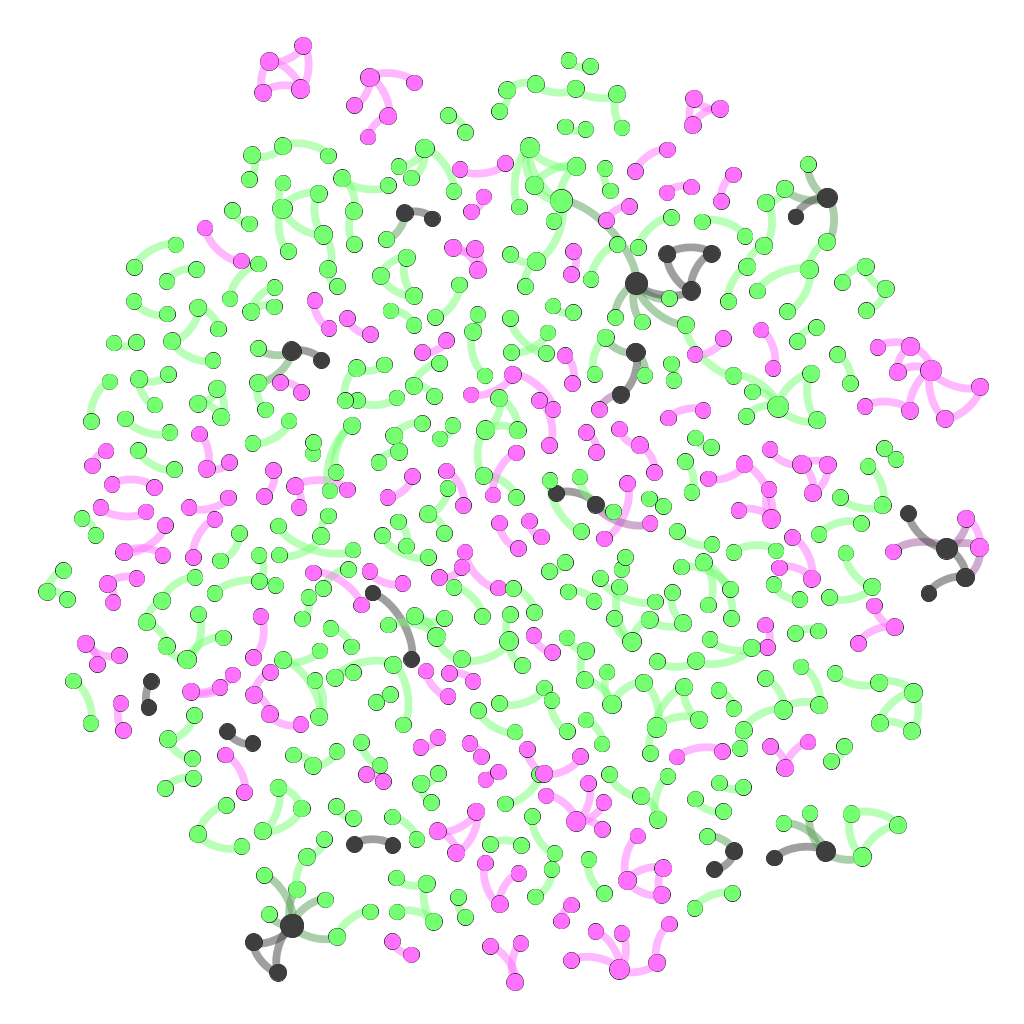
\includegraphics[width=5cm, height=5cm]{S42000.png}
  \endminipage\hfill
  \minipage{0.32\textwidth}
    \textbf{2005}\\
    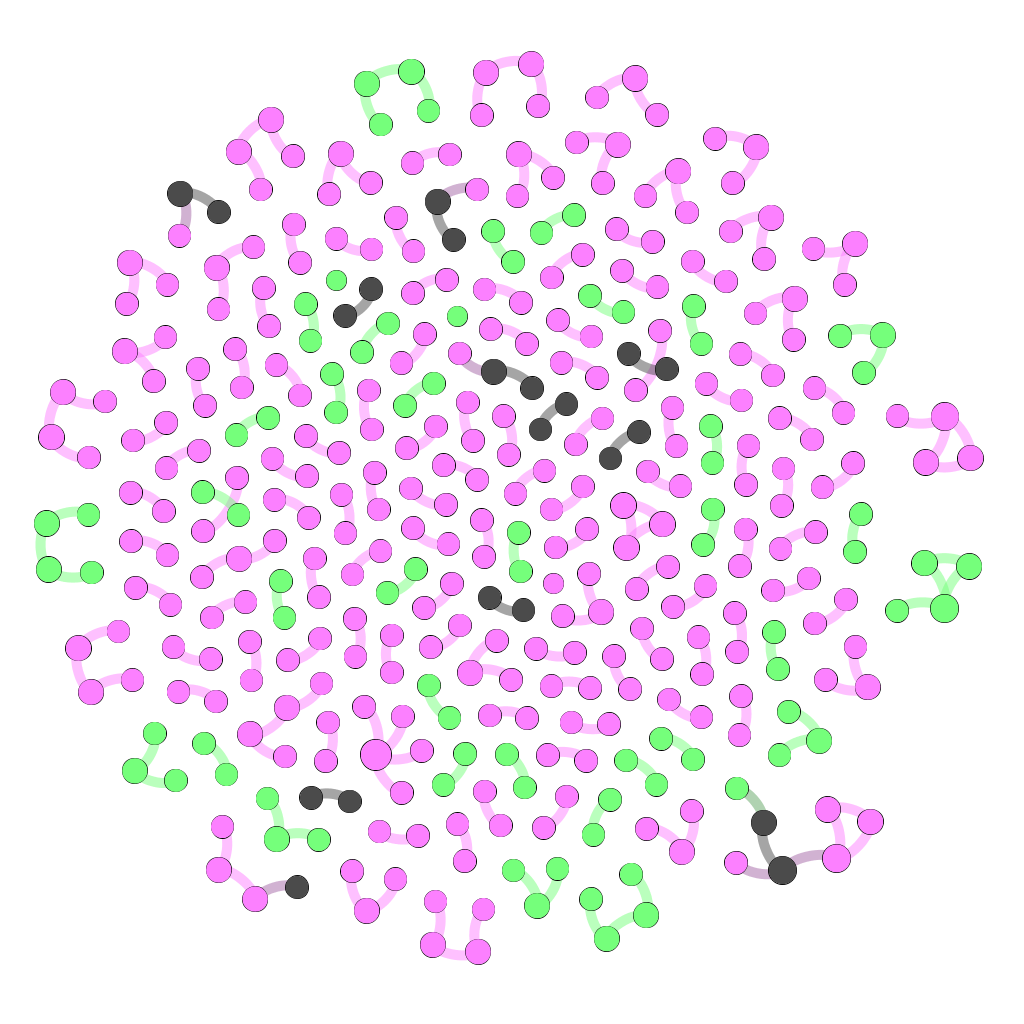
\includegraphics[width=5cm, height=5cm]{S42005.png}
  \endminipage\hfill
  \minipage{0.32\textwidth}
    \textbf{2010}\\
    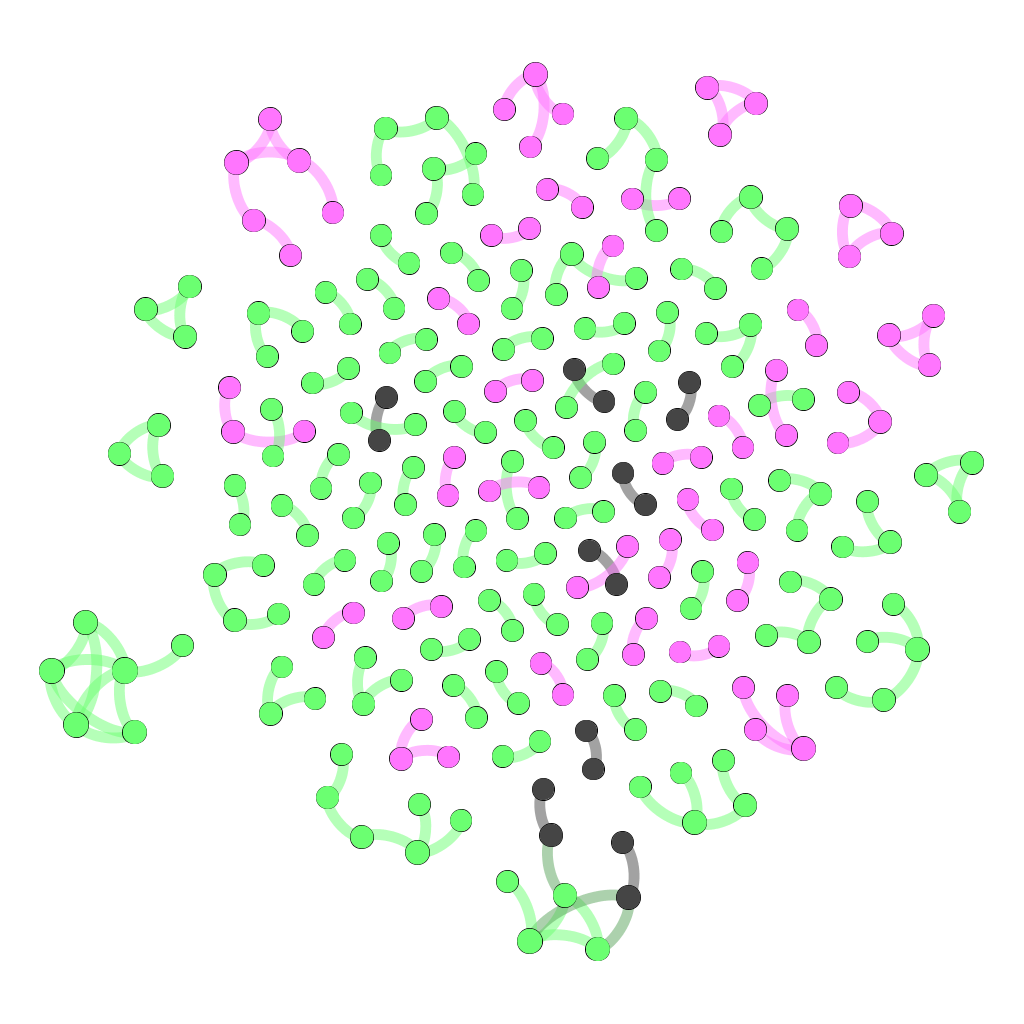
\includegraphics[width=5cm, height=5cm]{S42010.png}
  \endminipage\hfill
  \minipage{0.32\textwidth}%
    \textbf{2015}\\
    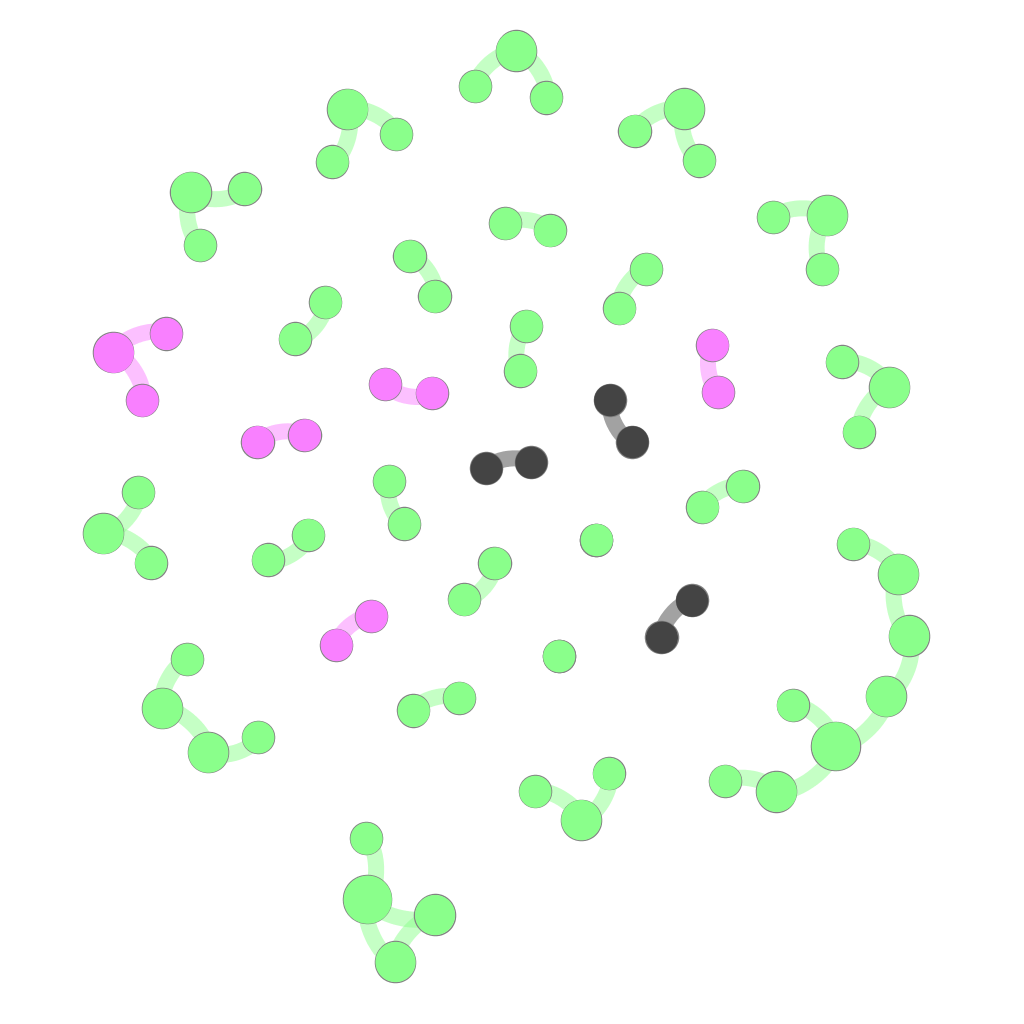
\includegraphics[width=5cm, height=5cm]{S42015.png}
  \endminipage
  \caption{Evolution of the nongiant components in the network}
  \label{fig:s4}
\end{figure}

This figure depicts the development of the nongiant components in the direct collaboration network. Similarly to Figure 2A and Figure S3, green and magenta nodes represent faculty $F_i$ in BIO and CS department, respectively, while black nodes represent faculty $F_i$ in the XD group. 

Notably, the number of nodes and links decreases significantly from 1990 to 2015. If in the year 1990, due to the lack of cross-disciplinary collaborations, there are some local strong groups of internal collaboration. In the 1991-1995 period, the network also presents the establishment of cross-disciplinary collaboration. However, those groups of collaboration are still local and disjointed. From 2000 to 2010, when the size of local disjointed groups increases and there were links connecting these groups so that they joined to the giant component and disappear in the network of nongiant in those years. Finally, in the year 2015, there are only a few faculties who are left out of the giant robust component.




\bigskip   % leave some empty space (optional)

\end{document}

